\documentclass[10pt]{article}
\usepackage[margin=0.85in]{geometry}
\usepackage{amsmath,amssymb}
\usepackage{enumitem}
\usepackage{xcolor}
\usepackage{tikz}
\usetikzlibrary{arrows.meta,positioning,calc,shapes.geometric,fit,backgrounds,matrix}
\setlist{nosep,leftmargin=1.4em}
\usepackage[hidelinks]{hyperref}
\usepackage{parskip}
\newcommand{\A}{\mathcal{A}}
\newcommand{\bX}{\mathbf{X}}
\newcommand{\bx}{\mathbf{x}}
\newcommand{\bn}{\mathbf{n}}
\newcommand{\bw}{\mathbf{w}}
\newcommand{\Sset}{\mathcal{S}}
\newcommand{\bos}{\texttt{[BOS]}}
\newcommand{\eos}{\texttt{[EOS]}}
\newcommand{\C}{\mathbb{C}}
% Inline markers tying audit findings (red) and proposed fixes (green) to the
% architecture figures in Section 8.
\DeclareRobustCommand{\flagmk}[1]{\tikz[baseline=-0.62ex]{\node[circle,draw=red!70!black,
  fill=red!12,text=red!70!black,inner sep=0.8pt,font=\tiny\bfseries]{#1};}}
\DeclareRobustCommand{\fixmk}[1]{\tikz[baseline=-0.62ex]{\node[circle,draw=green!45!black,
  fill=green!14,text=green!45!black,inner sep=0.8pt,font=\tiny\bfseries]{#1};}}
\title{\vspace{-2.5em}\textbf{SoundReg: working brief (problem, math, experiment)}}
\date{\vspace{-2em}}
\begin{document}
\maketitle

\begin{figure}[t]
\centering
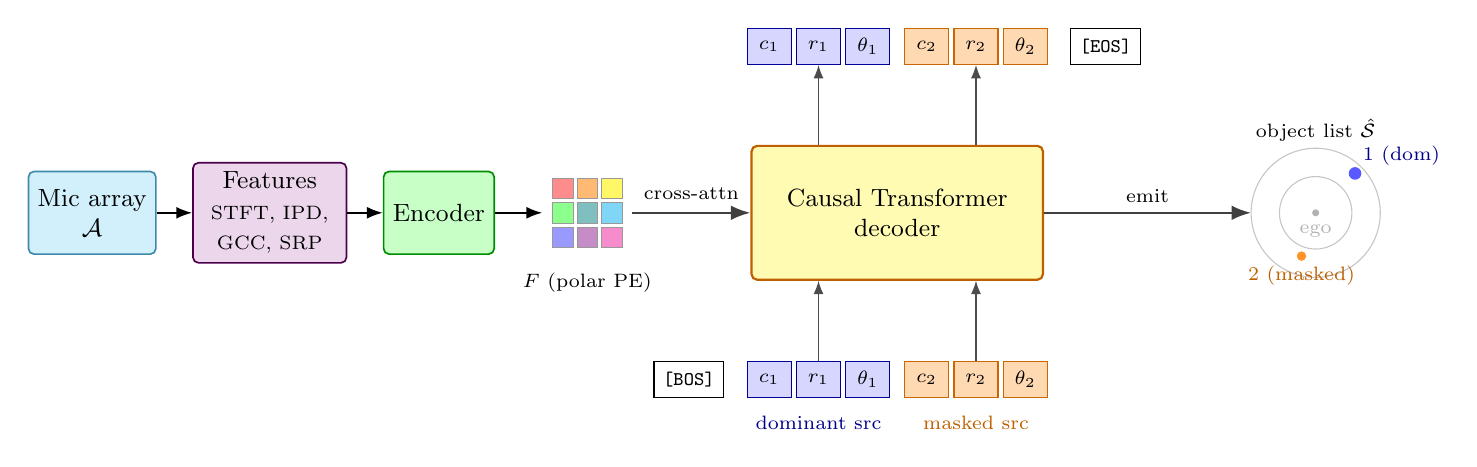
\begin{tikzpicture}[font=\small,>=Latex,
  mic/.style={draw=cyan!65!black,line width=0.6pt,rounded corners=2pt,align=center,fill=cyan!18,minimum height=1.05cm},
  fea/.style={draw=violet!60!black,line width=0.6pt,rounded corners=2pt,align=center,fill=violet!16,minimum height=1.05cm},
  enc/.style={draw=green!55!black,line width=0.6pt,rounded corners=2pt,align=center,fill=green!22,minimum height=1.05cm},
  dec/.style={draw=orange!75!black,line width=0.8pt,rounded corners=2pt,align=center,fill=yellow!30,minimum height=1.7cm},
  tok/.style={draw,minimum width=0.56cm,minimum height=0.46cm,font=\scriptsize,fill=white},
  domtok/.style={tok,draw=blue!60!black,fill=blue!16},
  masktok/.style={tok,draw=orange!80!black,fill=orange!30}]

  \node[mic,minimum width=1.5cm] (mic) {Mic array\\$\A$};
  \node[fea,right=0.45cm of mic,minimum width=1.95cm] (feat) {Features\\{\scriptsize STFT, IPD,}\\{\scriptsize GCC, SRP}};
  \node[enc,right=0.45cm of feat,minimum width=1.3cm] (enc) {Encoder};
  \matrix[right=0.6cm of enc,column sep=1.2pt,row sep=1.2pt,
          every node/.style={draw=black!40,line width=0.3pt,minimum size=0.26cm}] (Fg)
   {\node[fill=red!45]{};   & \node[fill=orange!55]{}; & \node[fill=yellow!60]{}; \\
    \node[fill=green!45]{}; & \node[fill=teal!50]{};   & \node[fill=cyan!50]{};   \\
    \node[fill=blue!40]{};  & \node[fill=violet!45]{}; & \node[fill=magenta!45]{};\\};
  \node[below=2pt of Fg,font=\scriptsize] {$F$ (polar PE)};
  \node[dec,right=1.5cm of Fg,minimum width=3.7cm] (dec) {Causal Transformer\\decoder};
  \draw[->,line width=0.6pt](mic)--(feat);
  \draw[->,line width=0.6pt](feat)--(enc);
  \draw[->,line width=0.6pt](enc)--(Fg);
  \draw[->,line width=0.9pt,draw=black!75](Fg.east)--node[above=1pt,font=\scriptsize]{cross-attn}(dec.west);

  % input tokens below decoder, vertical arrows up into the decoder
  \node[domtok] (i2) at ($(dec.south)+(-1.0cm,-1.25cm)$) {$r_1$};
  \node[domtok,left=1.5pt of i2]  (i1) {$c_1$};
  \node[domtok,right=1.5pt of i2] (i3) {$\theta_1$};
  \node[tok,left=8pt of i1]       (i0) {$\bos$};
  \node[masktok] (i5) at ($(dec.south)+(1.0cm,-1.25cm)$) {$r_2$};
  \node[masktok,left=1.5pt of i5]  (i4) {$c_2$};
  \node[masktok,right=1.5pt of i5] (i6) {$\theta_2$};
  \draw[->,draw=black!70] (i2.north) -- ($(dec.south)+(-1.0cm,0)$);
  \draw[->,draw=black!70] (i5.north) -- ($(dec.south)+(1.0cm,0)$);
  \node[font=\scriptsize,blue!55!black]   at ($(i2.south)+(0,-0.32)$) {dominant src};
  \node[font=\scriptsize,orange!75!black] at ($(i5.south)+(0,-0.32)$) {masked src};

  % output tokens above decoder, vertical arrows out of the decoder
  \node[domtok] (o2) at ($(dec.north)+(-1.0cm,1.25cm)$) {$r_1$};
  \node[domtok,left=1.5pt of o2]  (o1) {$c_1$};
  \node[domtok,right=1.5pt of o2] (o3) {$\theta_1$};
  \node[masktok] (o5) at ($(dec.north)+(1.0cm,1.25cm)$) {$r_2$};
  \node[masktok,left=1.5pt of o5]  (o4) {$c_2$};
  \node[masktok,right=1.5pt of o5] (o6) {$\theta_2$};
  \node[tok,right=8pt of o6] (o7) {$\eos$};
  \draw[->,draw=black!70] ($(dec.north)+(-1.0cm,0)$) -- (o2.south);
  \draw[->,draw=black!70] ($(dec.north)+(1.0cm,0)$) -- (o5.south);

  % decoded sequence becomes the BEV object list, connected to the decoder
  \begin{scope}[shift={($(dec.east)+(3.45cm,0)$)}]
    \draw[gray!45](0,0) circle (0.82);
    \draw[gray!45](0,0) circle (0.46);
    \fill[gray!60](0,0) circle (0.045) node[below=1pt,font=\scriptsize]{ego};
    \fill[blue!65](0.5,0.5) circle (0.08) node[above right=-1pt,font=\scriptsize,blue!55!black]{1 (dom)};
    \fill[orange!85](-0.18,-0.55) circle (0.06) node[below=0pt,font=\scriptsize,orange!75!black]{2 (masked)};
    \node[font=\scriptsize] at (0,1.05) {object list $\hat\Sset$};
  \end{scope}
  \draw[->,line width=0.9pt,draw=black!75]
    (dec.east) -- node[above=0pt,font=\scriptsize]{emit} ($(dec.east)+(2.63cm,0)$);
\end{tikzpicture}
\caption{SoundReg. Audio is encoded once into scene features $F$; a causal decoder
cross-attends to $F$ and emits sounding objects one at a time in dominance order.
The dominant source (blue) is emitted first; conditioning on it is intended to let the
decoder recover the masked source (orange) that a parallel detector, working from
the full mixture, tends to drop.}
\label{fig:arch}
\end{figure}


\section*{1. Problem}
From a short multichannel window $\A$ of one ego-mounted microphone array (audio
only, no vision at inference), output the set of road users currently making
task-relevant sound, each as (class, range, azimuth) in the bird's-eye-view (BEV)
plane:
\[
\mathcal{S}=\{(c_i,r_i,\theta_i)\}_{i=1}^{N},\qquad N \text{ unknown and variable.}
\]
This is the object list a planner already consumes from LiDAR and camera, not the
single direction that classical localization or SELD produce. Sound is useful
because it is not line-of-sight bound (sources audible around corners, before they
are visible). LiDAR gives accurate positions for in-sight objects and is used as
the training label there.

\section*{2. Idea (one sentence)}
Masking is the acoustic analog of occlusion: a loud source hides weaker concurrent
sources in the time-frequency (TF) bins it dominates, so generate objects loudest
first (dominance order) and condition each one on those already emitted. The
ordering is an inductive bias that should help a finite-capacity model recover
low-SNR masked sources; expect the benefit to be largest on hard cases and in the
small-data regime, and to shrink with more data.

\section*{3. Signal model and the quantities that matter}
Stacked-channel STFT of the mixture, with per-source array images $\bx_i$ and noise
$\bn$:
\begin{equation}
\bX(t,f)=\sum_{i=1}^{N}\bx_i(t,f)+\bn(t,f),\qquad E_i=\sum_{t,f}\|\bx_i(t,f)\|^2 .
\end{equation}
Difficulty of source $j$ seen against all others (what a parallel detector faces),
and after a set $C$ of sources is accounted for:
\begin{equation}
\mathrm{SNR}_j(\varnothing)=\frac{E_j}{\sum_{i\neq j}E_i^{(j)}+E_n^{(j)}},
\qquad
\mathrm{SNR}_j(C)=\frac{E_j}{\sum_{i\notin C\cup\{j\}}E_i^{(j)}+E_n^{(j)}}\ \geq\ \mathrm{SNR}_j(\varnothing),
\end{equation}
where $E_i^{(j)},E_n^{(j)}$ are interferer/noise energy in $j$'s TF support. The
useful quantity is the \emph{headroom} $\mathrm{SNR}_j(C)-\mathrm{SNR}_j(\varnothing)$:
zero when nothing masks $j$, large when $C$ holds $j$'s maskers. $\mathrm{SNR}_j(C)$
is an oracle (perfect removal of $C$); the model only approaches it by conditioning
on emitted tokens. Generation order is set by a dominance score (steered-response
power), emitted in descending $d_i$:
\begin{equation}
d_i=\sum_{t,f}\big|\bw(r_i,\theta_i)^{\!\mathsf{H}}\bX(t,f)\big|^2 .
\end{equation}

\section*{4. Model}
Each object is three tokens: class $c_i$, quantized range $t^r_i$, quantized
azimuth $t^\theta_i$ (separate vocabulary per axis; azimuth finer than range). A
scene in dominance order $\pi$ and its likelihood:
\begin{equation}
O_\pi=[\,\bos,(c,t^r,t^\theta)_{\pi(1)},\dots,(c,t^r,t^\theta)_{\pi(N)},\eos\,],
\end{equation}
\begin{equation}
p_\Theta(O_\pi\mid\A)=p_\Theta(\eos\mid h_{N+1})\prod_{i=1}^{N}
p_\Theta(c_i\mid h_i)\,p_\Theta(t^r_i\mid c_i,h_i)\,p_\Theta(t^\theta_i\mid c_i,t^r_i,h_i),
\end{equation}
where $h_i$ summarizes the scene features $F$ and the objects already emitted.
Train by teacher forcing with one cross-entropy:
\begin{equation}
\mathcal{L}=-\sum_{i=1}^{N}\big[\log p_\Theta(c_i\mid h_i)+\log p_\Theta(t^r_i\mid c_i,h_i)+\log p_\Theta(t^\theta_i\mid c_i,t^r_i,h_i)\big]-\log p_\Theta(\eos\mid h_{N+1}).
\end{equation}
Pieces to implement:
\begin{itemize}
\item Encoder: features $\A\to$ STFT, inter-channel phase difference (IPD),
GCC-PHAT, optional SRP map on the polar grid $\to$ $F$ with a polar positional
encoding (separate range and azimuth embeddings).
\item Decoder: causal Transformer, cross-attends to $F$, token-type masking (class
steps emit class tokens, location steps emit location tokens).
\item Cardinality: \eos\ ends the sequence (no fixed query count, no threshold).
\item Inference: greedy/beam for main numbers; sample $S$ sequences and cluster for
existence/uncertainty.
\end{itemize}
Section~8 documents the architecture as actually built on the Acoustic-BEV data
(Fig.~\ref{fig:arch-v1}), the audit of that instantiation, and the proposed
revision (Fig.~\ref{fig:arch-v2}).

\section*{5. Data and ground truth you need}
\begin{itemize}
\item Real array+LiDAR driving data (all line-of-sight). Decide and record: array
geometry/channels, polar grid ($N_\theta,N_r,r_{\max}$), train/val/test split.
\item Ground truth = objects \emph{actually emitting} task-relevant sound, with
class and position. Sound-activity must be annotated independently of the detector
(else the evaluation is circular). Position from the LiDAR track.
\item Per-source SNR (for stratifying recall): exact in simulation; on real LOS
data estimate by beamforming toward each labeled source.
\item NLOS: (i) simulated NLOS scenes with known positions mixed into training of
every set-prediction model, (ii) a small hand-annotated real NLOS test set. Scoped
demo, not a benchmark.
\end{itemize}

\section*{6. Experiment (run in this order)}
\textbf{Baselines (parallel):} GCC/SRP peak picking; SELD-style class+DOA; polar
heatmap + peak extraction; query-set predictor (DETR / Sound3DVDet style). SoundReg
is the only sequential one.

\textbf{Metrics:} match prediction to GT by class + polar-distance threshold; report
F1, cardinality error (\,$|\hat N-N|$\,), range/azimuth MAE. Report mean $\pm$ std
over several seeds.

\textbf{Headline test (do this first).} Recall stratified by per-source SNR and by
number of concurrent sources, SoundReg vs each baseline.
\begin{itemize}
\item Prediction: SoundReg's recall advantage \emph{grows} as SNR drops and overlap
rises.
\item Falsifier: a flat advantage. If the gap does not grow at low SNR, the masking
idea is wrong, stop here.
\item Watch the opposite failure: the decoder can fire \eos\ early and \emph{drop}
quiet masked sources, which shows up as \emph{worse} low-SNR recall. Monitor \eos\
calibration; also report a length-controlled decoding variant.
\end{itemize}

\textbf{Ablations (each isolates one thing).}
\begin{itemize}
\item Order: dominance vs distance vs azimuth-sweep vs random vs oracle
masking-order (upper bound).
\item Conditioning: full vs context-masked decoder (predict each object without
seeing previously emitted objects). This is the cleanest test that conditioning,
not tokenization, does the work.
\item Dominance estimator: beamformer power vs oracle energy vs SNR.
\item NLOS: train with vs without simulated NLOS data; compare NLOS detection rate
against the query baseline given the \emph{same} NLOS targets.
\item Soft target: one-bin Gaussian vs hard label.
\end{itemize}

\textbf{Second prediction (data scaling).} The advantage should shrink as training
data grows (it is an inductive bias, not an information gain). Run a small
data-fraction sweep against the query baseline.

\section*{7. The data on hand, and what to prepare}
Each sample (one \texttt{token}) carries:
{\small
\begin{verbatim}
items[token] = {
  "stft":     ndarray (64, F, T)   # 32 mics; complex split to 64 real ch; encoder input
  "audio":    ndarray (T, 32)      # optional raw multichannel
  "ann":      [ {"center":[x,y,z], "wlh":[w,l,h]}, ... ]  # sounding objects only
  "lidar":    ndarray (N, 3)       # box-position source; not used at inference
  "velocity": {lin_x,lin_y,lin_z, ang_x,ang_y,ang_z}     # ego motion (optional)
  "timestamp", "scene_name"
}
\end{verbatim}
}
The annotated boxes are the sounding objects; silent objects are simply not
annotated, so there is nothing to detect for them. A single class is used, so the
class token $c_i$ in Eqs.~(4) to (6) is constant and drops out: a target token is
just $(r,\theta)$. Microphone positions come from a separate XML file (the array
geometry).

\textbf{Preparation. Each sample becomes one (features, ordered target sequence) pair:}
\begin{enumerate}
\item Mic geometry: parse the XML into microphone positions $\in\mathbb{R}^{M\times3}$. One-time.
\item Polar grid: fix $r_{\max}$, $N_r$, $N_\theta$. This is the target vocabulary.
\item Steering vectors: precompute $w(r,\theta)$ per grid cell and frequency from the geometry. One-time.
\item Features: from \texttt{stft}, build log-magnitude and inter-channel phase difference (optionally GCC-PHAT). Encoder input.
\item Targets: each \texttt{ann} center $[x,y]$ gives $r=\sqrt{x^2+y^2}$, $\theta=\mathrm{atan2}(y,x)$, quantized to a $(r,\theta)$ bin.
\item Order: dominance $d_i=\sum_{t,f}|w(r_i,\theta_i)^{\mathsf H}\mathbf{X}(t,f)|^2$ per box; sort high to low; prepend \bos, append \eos.
\item SNR (evaluation only): beamform toward each source, estimate its SNR, store it with the sample to stratify recall.
\end{enumerate}
After step 7 each sample is $[\bos,(r,\theta)_1,\dots,(r,\theta)_N,\eos]$ paired with
its features, and the model trains directly on it.

\section*{8. Implementation on Acoustic-BEV: as built, audit, revision}

\textbf{As built (v1, Fig.~\ref{fig:arch-v1}).} The encoder reuses the MoG-slot
network's front end from \texttt{Acoustic-BEV/src/evidential} unchanged: SpeedFiLM
conditions the stacked re/im STFT $(64{\times}19{\times}84)$ on ego speed, the conv
trunk ends in a $(100{\times}19{\times}360)$ angular feature map, and the same
tokenization the K-slot head used (mean over $T$, angular axis becomes the
sequence) yields 360 memory tokens. Only the head changes: where $K$ learned
queries attended once, a causal Transformer decoder cross-attends and emits
$(t^r,t^\theta)$ pairs in dominance order until \eos. Single class, so the class
token of Eqs.~(4)\,to\,(6) drops out. Trained with Eq.~(6); scored with the
benchmark matcher ($5^\circ$, $5^\circ{+}5$\,m gates).

\textbf{Audit: where v1 under-serves the hypothesis.} The red markers in
Fig.~\ref{fig:arch-v1} locate each problem on the component that causes it.
\begin{itemize}
\item \flagmk{1} \textbf{Time is destroyed before conditioning can use it.} The
mean over $T$ integrates out exactly the TF glimpses (frames where the masker is
weak) that make a masked source recoverable. The hypothesis needs them downstream.
\item \flagmk{2} \textbf{Geometry is unused in the features, and range has no
axis.} The ``angular'' axis is a learned $1{\times}1$ reinterpretation of channels;
nothing ties token $k$ to azimuth $k$, and range must hide inside channel content.
Meanwhile exact steering vectors are already computed, but only for ordering.
\item \flagmk{3} \textbf{Vocabulary too coarse for the gate.} $5^\circ$ azimuth bins
against a $5^\circ$ matching gate donate up to $2.5^\circ$ of pure quantization
error; the continuous-output baseline reports mAAE $2.5^\circ$.
\item \flagmk{4} \textbf{No operating point.} Baselines tune their threshold for F1
on val; \eos\ gives SoundReg no precision/recall knob, and early \eos\ suppresses
recall on precisely the quiet sources under study.
\item \flagmk{5} \textbf{Architecture reused, weights not.} Training the trunk from
scratch forfeits a phase-to-angle mapping that trained MoG checkpoints already
contain, on a dataset too small to relearn it comfortably.
\end{itemize}
Two further, smaller issues do not appear in the figure: dominance is a noisy
ordering label near ties (and the free-field steering ignores spatial aliasing
above ${\sim}1.7$\,kHz and car-body shadowing), and with $N\!\le\!3$ the loss
allocates almost no gradient to the last-emitted quiet objects.

\textbf{Proposed revision (v2, Fig.~\ref{fig:arch-v2}).} Each fix is one green
marker, one Settings-level change, one ablation.
\begin{itemize}
\item \fixmk{1} Replace the mean with \textbf{attention pooling over $T$}: a
learned query per angular position keeps access to per-frame evidence.
\item \fixmk{2} Add the \textbf{geometric feature path}: steering vectors from the
mic XML produce SRP maps on the $(r,\theta)$ target grid; a small conv head turns
them into polar tokens (range axis restored, azimuth grounded) concatenated into
the decoder memory.
\item \fixmk{3} \textbf{Azimuth vocabulary $72\!\to\!240$} ($1.5^\circ$ bins); the
vocabulary is tiny either way, the quantization floor drops below the gate.
\item \fixmk{4} Report \textbf{length-controlled decoding} next to greedy and track
\eos\ calibration from epoch~1, so cardinality failures are visible and separable
from localization failures.
\item \fixmk{5} \textbf{Initialize the trunk from a trained MoG checkpoint}
(frozen for the first epochs), turning architectural reuse into actual transfer.
\end{itemize}
The decoder, the dominance ordering, the single cross-entropy, and \eos\
cardinality are unchanged: v2 revises only how evidence reaches the decoder, not
the formulation.

\begin{figure}[p]
\centering
\resizebox{\textwidth}{!}{%
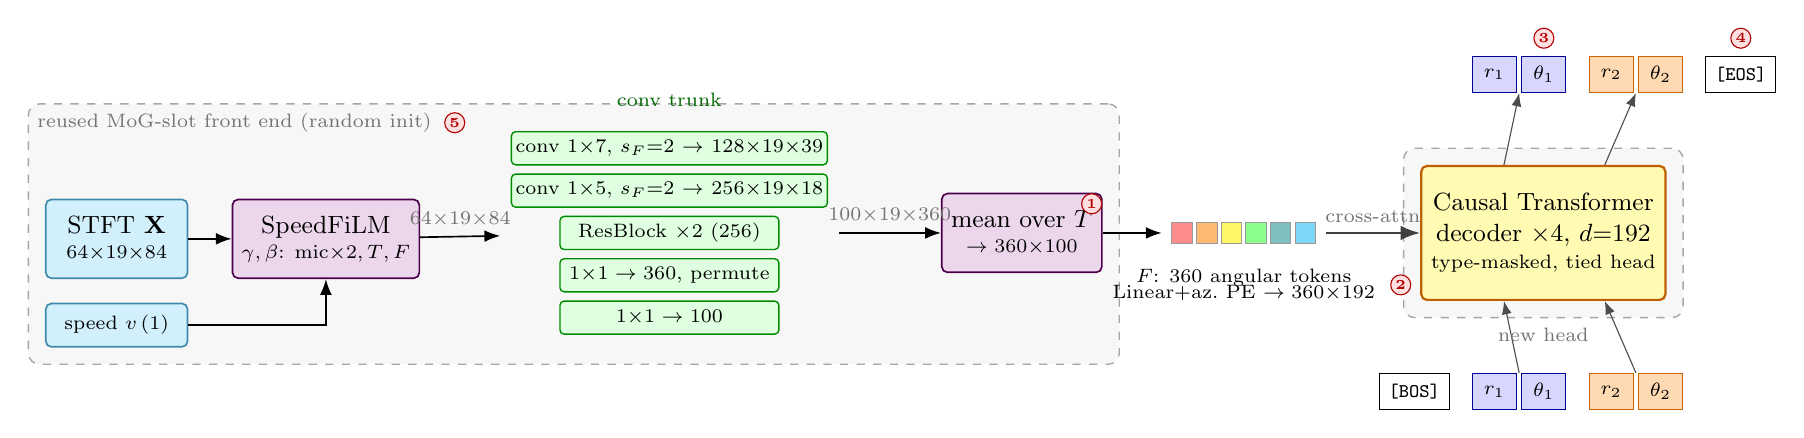
\begin{tikzpicture}[font=\small,>=Latex,
  mic/.style={draw=cyan!65!black,line width=0.6pt,rounded corners=2pt,align=center,fill=cyan!18},
  fea/.style={draw=violet!60!black,line width=0.6pt,rounded corners=2pt,align=center,fill=violet!16},
  dec/.style={draw=orange!75!black,line width=0.8pt,rounded corners=2pt,align=center,fill=yellow!30},
  stage/.style={draw=green!55!black,line width=0.5pt,rounded corners=1.5pt,fill=green!12,
                font=\scriptsize,minimum width=2.78cm,minimum height=0.42cm,inner sep=1.5pt,align=center},
  tok/.style={draw,minimum width=0.56cm,minimum height=0.46cm,font=\scriptsize,fill=white},
  domtok/.style={tok,draw=blue!60!black,fill=blue!16},
  masktok/.style={tok,draw=orange!80!black,fill=orange!30},
  cell/.style={draw=black!40,line width=0.3pt,minimum size=0.26cm},
  shp/.style={font=\scriptsize,text=black!55},
  flag/.style={circle,draw=red!70!black,fill=red!12,text=red!70!black,inner sep=0.8pt,font=\tiny\bfseries},
  grp/.style={draw=black!35,dashed,line width=0.5pt,rounded corners=4pt,fill=black!3,inner xsep=6pt,inner ysep=12pt}]

  % ---------- inputs ----------
  \node[mic,minimum width=1.8cm,minimum height=1.0cm] (stft) {STFT $\bX$\\[-2pt]{\scriptsize$64{\times}19{\times}84$}};
  \node[mic,minimum width=1.8cm,minimum height=0.55cm,below=0.3cm of stft] (spd) {\scriptsize speed $v$\,$(1)$};

  % ---------- FiLM ----------
  \node[fea,minimum width=2.0cm,minimum height=1.0cm,right=0.55cm of stft] (film)
    {SpeedFiLM\\[-2pt]{\scriptsize$\gamma,\beta$: mic${\times}2$,\,$T$,\,$F$}};

  % ---------- trunk stack ----------
  \node[stage,right=1.15cm of film,yshift=1.15cm] (t1) {conv $1{\times}7$, $s_F{=}2$ $\to$ $128{\times}19{\times}39$};
  \node[stage,below=0.10cm of t1] (t2) {conv $1{\times}5$, $s_F{=}2$ $\to$ $256{\times}19{\times}18$};
  \node[stage,below=0.10cm of t2] (t3) {ResBlock $\times2$ (256)};
  \node[stage,below=0.10cm of t3] (t4) {$1{\times}1\to360$, permute};
  \node[stage,below=0.10cm of t4] (t5) {$1{\times}1\to100$};
  \begin{scope}[on background layer]
    \node[draw=green!55!black,line width=0.6pt,rounded corners=2pt,fill=green!22,
          fit=(t1)(t5),inner sep=3.5pt] (trunk) {};
  \end{scope}
  \node[font=\scriptsize,green!40!black,above=1.5pt of trunk] {conv trunk};

  % ---------- tokenize ----------
  \node[fea,minimum width=1.7cm,minimum height=1.0cm,right=1.30cm of trunk] (pool)
    {mean over $T$\\[-2pt]{\scriptsize$\to 360{\times}100$}};
  \node[flag] at ($(pool.north east)+(-0.14,-0.14)$) {1};

  % ---------- memory strip ----------
  \matrix[ampersand replacement=\&,right=0.75cm of pool,column sep=1.2pt,
          every node/.style={cell}] (mem)
   {\node[fill=red!45]{};   \& \node[fill=orange!55]{}; \& \node[fill=yellow!60]{}; \&
    \node[fill=green!45]{}; \& \node[fill=teal!50]{};   \& \node[fill=cyan!50]{};   \\};
  \node[below=2pt of mem,font=\scriptsize,align=center] (memlab)
    {$F$: 360 angular tokens\\[-2pt]Linear${+}$az.\ PE $\to 360{\times}192$};
  \node[flag,right=2pt of memlab] {2};

  % ---------- decoder ----------
  \node[dec,minimum width=3.1cm,minimum height=1.7cm,right=1.20cm of mem] (dcd)
    {Causal Transformer\\decoder $\times4$, $d{=}192$\\[-1pt]{\scriptsize type-masked, tied head}};

  % ---------- input/output token strips ----------
  \node[domtok]  (i2) at ($(dcd.south)+(-0.62cm,-1.15cm)$) {$r_1$};
  \node[tok,left=8pt of i2] (i0) {\bos};
  \node[domtok,right=1.5pt of i2] (i3) {$\theta_1$};
  \node[masktok,right=8pt of i3] (i4) {$r_2$};
  \node[masktok,right=1.5pt of i4] (i5) {$\theta_2$};
  \draw[->,draw=black!70] ($(i2.north)!0.5!(i3.north)$) -- ($(dcd.south)+(-0.5cm,0)$);
  \draw[->,draw=black!70] ($(i4.north)!0.5!(i5.north)$) -- ($(dcd.south)+(0.78cm,0)$);

  \node[domtok]  (o2) at ($(dcd.north)+(-0.62cm,1.15cm)$) {$r_1$};
  \node[domtok,right=1.5pt of o2] (o3) {$\theta_1$};
  \node[masktok,right=8pt of o3] (o4) {$r_2$};
  \node[masktok,right=1.5pt of o4] (o5) {$\theta_2$};
  \node[tok,right=8pt of o5] (o6) {\eos};
  \draw[->,draw=black!70] ($(dcd.north)+(-0.5cm,0)$) -- ($(o2.south)!0.5!(o3.south)$);
  \draw[->,draw=black!70] ($(dcd.north)+(0.78cm,0)$) -- ($(o4.south)!0.5!(o5.south)$);
  \node[flag,above=2.5pt of o3] {3};
  \node[flag,above=2.5pt of o6] {4};

  % ---------- arrows ----------
  \draw[->,line width=0.6pt] (stft) -- (film);
  \draw[->,line width=0.6pt] (spd.east) -| ($(film.south)+(0,-0.0cm)$);
  \draw[->,line width=0.6pt] (film) -- node[shp,above]{\scriptsize$64{\times}19{\times}84$} (trunk);
  \draw[->,line width=0.6pt] (trunk) -- node[shp,above]{\scriptsize$100{\times}19{\times}360$} (pool);
  \draw[->,line width=0.6pt] (pool) -- (mem);
  \draw[->,line width=0.9pt,draw=black!75] (mem.east) -- node[shp,above]{cross-attn} (dcd.west);

  % ---------- reuse / new containers ----------
  \begin{scope}[on background layer]
    \node[grp,fit=(film)(trunk)(pool)(spd),inner sep=6pt] (reused) {};
    \node[grp,fit=(dcd),inner sep=6pt] (newhead) {};
  \end{scope}
  \node[font=\scriptsize,black!55,anchor=north west] (reusedlab) at (reused.north west)
    {reused MoG-slot front end (random init)};
  \node[flag,right=1pt of reusedlab] {5};
  \node[font=\scriptsize,black!55,anchor=south] at ($(newhead.south)+(0,-0.42cm)$) {new head};
\end{tikzpicture}}
\caption{\textbf{As built (v1).} The implemented SoundReg on Acoustic-BEV: the
MoG-slot front end is reused unchanged up to its own tokenization (mean over $T$,
360 angular tokens), and only the head is new. Red markers locate the audit
findings of Section~8: \flagmk{1} time pooled out before conditioning,
\flagmk{2} learned angular axis with no range axis and no geometric grounding,
\flagmk{3} $5^\circ$ bins against the $5^\circ$ gate, \flagmk{4} no
precision/recall knob at \eos, \flagmk{5} reused architecture but not weights.}
\label{fig:arch-v1}
\end{figure}

\begin{figure}[p]
\centering
\resizebox{\textwidth}{!}{%
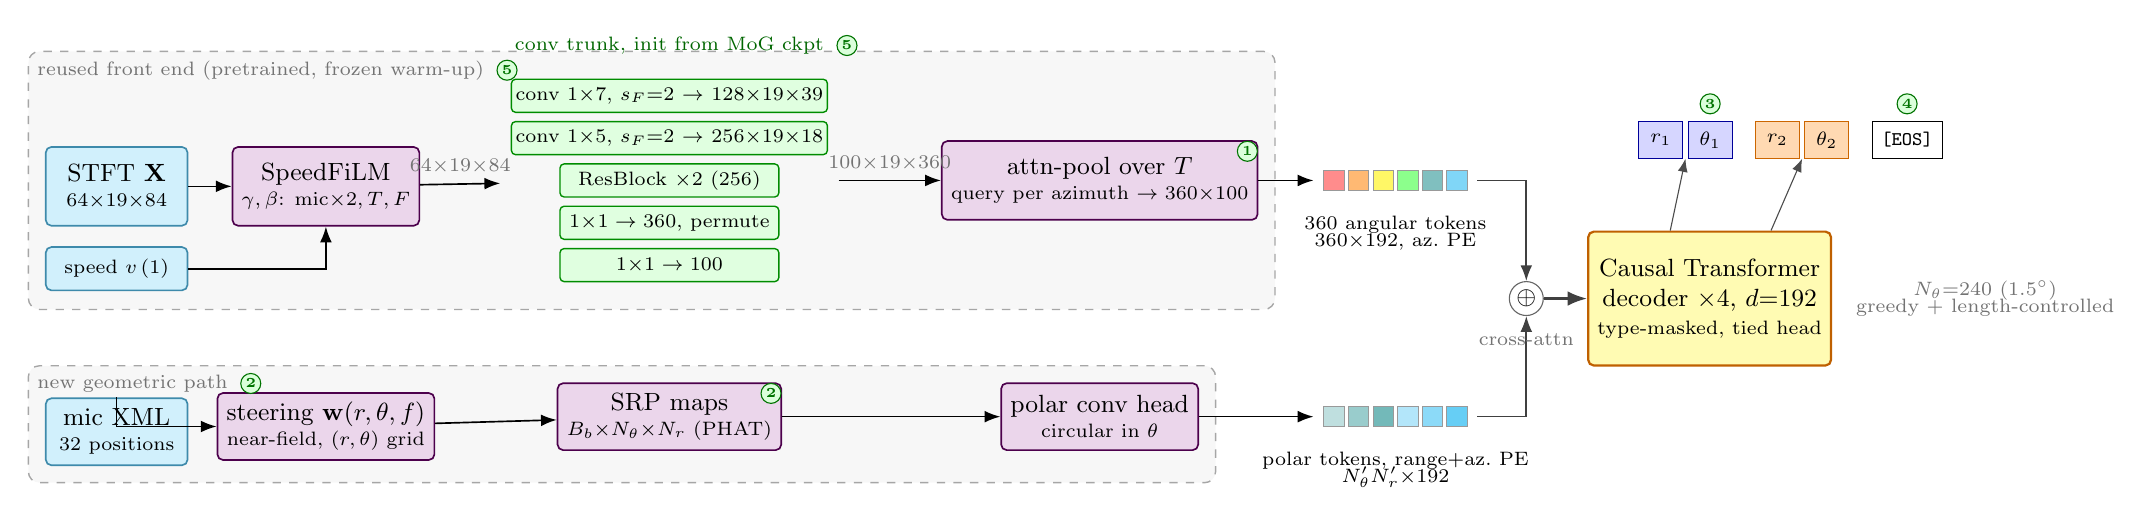
\begin{tikzpicture}[font=\small,>=Latex,
  mic/.style={draw=cyan!65!black,line width=0.6pt,rounded corners=2pt,align=center,fill=cyan!18},
  fea/.style={draw=violet!60!black,line width=0.6pt,rounded corners=2pt,align=center,fill=violet!16},
  dec/.style={draw=orange!75!black,line width=0.8pt,rounded corners=2pt,align=center,fill=yellow!30},
  stage/.style={draw=green!55!black,line width=0.5pt,rounded corners=1.5pt,fill=green!12,
                font=\scriptsize,minimum width=2.78cm,minimum height=0.42cm,inner sep=1.5pt,align=center},
  tok/.style={draw,minimum width=0.56cm,minimum height=0.46cm,font=\scriptsize,fill=white},
  domtok/.style={tok,draw=blue!60!black,fill=blue!16},
  masktok/.style={tok,draw=orange!80!black,fill=orange!30},
  cell/.style={draw=black!40,line width=0.3pt,minimum size=0.26cm},
  shp/.style={font=\scriptsize,text=black!55},
  fix/.style={circle,draw=green!45!black,fill=green!14,text=green!45!black,inner sep=0.8pt,font=\tiny\bfseries},
  grp/.style={draw=black!35,dashed,line width=0.5pt,rounded corners=4pt,fill=black!3,inner xsep=6pt,inner ysep=12pt}]

  % ---------- learned path (top) ----------
  \node[mic,minimum width=1.8cm,minimum height=1.0cm] (stft) {STFT $\bX$\\[-2pt]{\scriptsize$64{\times}19{\times}84$}};
  \node[mic,minimum width=1.8cm,minimum height=0.55cm,below=0.25cm of stft] (spd) {\scriptsize speed $v$\,$(1)$};
  \node[fea,minimum width=2.0cm,minimum height=1.0cm,right=0.55cm of stft] (film)
    {SpeedFiLM\\[-2pt]{\scriptsize$\gamma,\beta$: mic${\times}2$,\,$T$,\,$F$}};
  \node[stage,right=1.15cm of film,yshift=1.15cm] (t1) {conv $1{\times}7$, $s_F{=}2$ $\to$ $128{\times}19{\times}39$};
  \node[stage,below=0.10cm of t1] (t2) {conv $1{\times}5$, $s_F{=}2$ $\to$ $256{\times}19{\times}18$};
  \node[stage,below=0.10cm of t2] (t3) {ResBlock $\times2$ (256)};
  \node[stage,below=0.10cm of t3] (t4) {$1{\times}1\to360$, permute};
  \node[stage,below=0.10cm of t4] (t5) {$1{\times}1\to100$};
  \begin{scope}[on background layer]
    \node[draw=green!55!black,line width=0.6pt,rounded corners=2pt,fill=green!22,
          fit=(t1)(t5),inner sep=3.5pt] (trunk) {};
  \end{scope}
  \node[font=\scriptsize,green!40!black,above=1.5pt of trunk] (trunklab)
    {conv trunk, init from MoG ckpt};
  \node[fix,right=1pt of trunklab] {5};
  \node[fea,minimum width=1.9cm,minimum height=1.0cm,right=1.30cm of trunk] (pool)
    {attn-pool over $T$\\[-2pt]{\scriptsize query per azimuth $\to 360{\times}100$}};
  \node[fix] at ($(pool.north east)+(-0.14,-0.14)$) {1};
  \matrix[ampersand replacement=\&,right=0.70cm of pool,column sep=1.2pt,
          every node/.style={cell}] (mem)
   {\node[fill=red!45]{};   \& \node[fill=orange!55]{}; \& \node[fill=yellow!60]{}; \&
    \node[fill=green!45]{}; \& \node[fill=teal!50]{};   \& \node[fill=cyan!50]{};   \\};
  \node[below=2pt of mem,font=\scriptsize,align=center]
    {360 angular tokens\\[-2pt]$360{\times}192$, az.\ PE};

  % ---------- geometric path (bottom) ----------
  \node[mic,minimum width=1.8cm,minimum height=0.85cm,below=1.35cm of spd] (xml)
    {mic XML\\[-2pt]{\scriptsize 32 positions}};
  \node[fea,minimum width=2.0cm,minimum height=0.85cm,anchor=center] (steer) at ($(film.center)+(0,-3.05cm)$)
    {steering $\bw(r,\theta,f)$\\[-2pt]{\scriptsize near-field, $(r,\theta)$ grid}};
  \node[fea,minimum width=2.45cm,minimum height=0.85cm,anchor=center] (srp) at ($(trunk.center)+(0,-3.0cm)$)
    {SRP maps\\[-2pt]{\scriptsize$B_b{\times}N_\theta{\times}N_r$ (PHAT)}};
  \node[fix] at ($(srp.north east)+(-0.14,-0.14)$) {2};
  \node[fea,minimum width=1.9cm,minimum height=0.85cm,anchor=center] (pconv) at ($(pool.center)+(0,-3.0cm)$)
    {polar conv head\\[-2pt]{\scriptsize circular in $\theta$}};
  \matrix[ampersand replacement=\&,column sep=1.2pt,every node/.style={cell},anchor=center] (pmem) at ($(mem.center)+(0,-3.0cm)$)
   {\node[fill=teal!25]{};  \& \node[fill=teal!40]{};  \& \node[fill=teal!55]{}; \&
    \node[fill=cyan!30]{};  \& \node[fill=cyan!45]{};  \& \node[fill=cyan!60]{}; \\};
  \node[below=2pt of pmem,font=\scriptsize,align=center]
    {polar tokens, range${+}$az.\ PE\\[-2pt]$N_\theta' N_r'{\times}192$};

  % ---------- concat + decoder ----------
  \node[circle,draw=black!60,fill=white,inner sep=1pt,font=\small] (cat)
    at ($(mem.east)+(0.62cm,-1.5cm)$) {$\oplus$};
  \node[dec,minimum width=3.0cm,minimum height=1.7cm,right=0.55cm of cat] (dcd)
    {Causal Transformer\\decoder $\times4$, $d{=}192$\\[-1pt]{\scriptsize type-masked, tied head}};

  % ---------- output strip ----------
  \node[domtok]  (o2) at ($(dcd.north)+(-0.62cm,1.15cm)$) {$r_1$};
  \node[domtok,right=1.5pt of o2] (o3) {$\theta_1$};
  \node[masktok,right=8pt of o3] (o4) {$r_2$};
  \node[masktok,right=1.5pt of o4] (o5) {$\theta_2$};
  \node[tok,right=8pt of o5] (o6) {\eos};
  \draw[->,draw=black!70] ($(dcd.north)+(-0.5cm,0)$) -- ($(o2.south)!0.5!(o3.south)$);
  \draw[->,draw=black!70] ($(dcd.north)+(0.78cm,0)$) -- ($(o4.south)!0.5!(o5.south)$);
  \node[fix,above=2.5pt of o3] {3};
  \node[fix,above=2.5pt of o6] {4};
  \node[font=\scriptsize,black!55,align=center,anchor=west] at ($(dcd.east)+(0.18cm,0)$)
    {$N_\theta{=}240$ ($1.5^\circ$)\\[-2pt]greedy ${+}$ length-controlled};

  % ---------- arrows ----------
  \draw[->,line width=0.6pt] (stft) -- (film);
  \draw[->,line width=0.6pt] (spd.east) -| (film.south);
  \draw[->,line width=0.6pt] (film) -- node[shp,above]{\scriptsize$64{\times}19{\times}84$} (trunk);
  \draw[->,line width=0.6pt] (trunk) -- node[shp,above]{\scriptsize$100{\times}19{\times}360$} (pool);
  \draw[->,line width=0.6pt] (pool) -- (mem);
  \draw[->,line width=0.6pt] (xml) |- (steer.west);
  \draw[->,line width=0.6pt] (steer) -- (srp);
  \draw[->,line width=0.6pt] (srp) -- (pconv);
  \draw[->,line width=0.6pt] (pconv) -- (pmem);
  \draw[->,line width=0.6pt,draw=black!75] (mem.east) -| (cat.north);
  \draw[->,line width=0.6pt,draw=black!75] (pmem.east) -| (cat.south);
  \draw[->,line width=0.9pt,draw=black!75] (cat) -- (dcd.west);
  \node[shp,anchor=north] at ($(cat.south)+(0,-0.10)$) {cross-attn};

  % ---------- containers ----------
  \begin{scope}[on background layer]
    \node[grp,fit=(film)(trunk)(pool)(spd),inner sep=6pt] (reused) {};
    \node[grp,fit=(xml)(steer)(srp)(pconv),inner sep=6pt] (geom) {};
  \end{scope}
  \node[font=\scriptsize,black!55,anchor=north west] (reusedlab) at (reused.north west)
    {reused front end (pretrained, frozen warm-up)};
  \node[fix,right=1pt of reusedlab] {5};
  \node[font=\scriptsize,black!55,anchor=north west] (geomlab) at (geom.north west)
    {new geometric path};
  \node[fix,right=1pt of geomlab] {2};
\end{tikzpicture}}
\caption{\textbf{Proposed revision (v2).} Same formulation, better evidence flow.
Green markers are the fixes of Section~8: \fixmk{1} attention pooling preserves
per-frame (masking) structure, \fixmk{2} a geometric path turns the already
computed steering vectors into SRP polar tokens with an explicit range axis,
\fixmk{3} $1.5^\circ$ azimuth bins drop the quantization floor below the gate,
\fixmk{4} length-controlled decoding reported next to greedy with \eos\
calibration tracked, \fixmk{5} the trunk transfers trained MoG weights instead of
re-learning phase-to-angle from scratch. Decoder, ordering, loss, and \eos\
cardinality are unchanged.}
\label{fig:arch-v2}
\end{figure}

\end{document}